\documentclass[a4paper,11pt]{article}
\usepackage{pretty}

\title{Accounting for topography in impulse waves}
\author{\begin{tabular}{c c c}
    Louise & Cayroche \\
    Axel & Giboulot
\end{tabular}}

\coverhead{
    \centering
    
\includegraphics[width=0.4\linewidth]{media/lhe.png}
    \(\qquad\)
    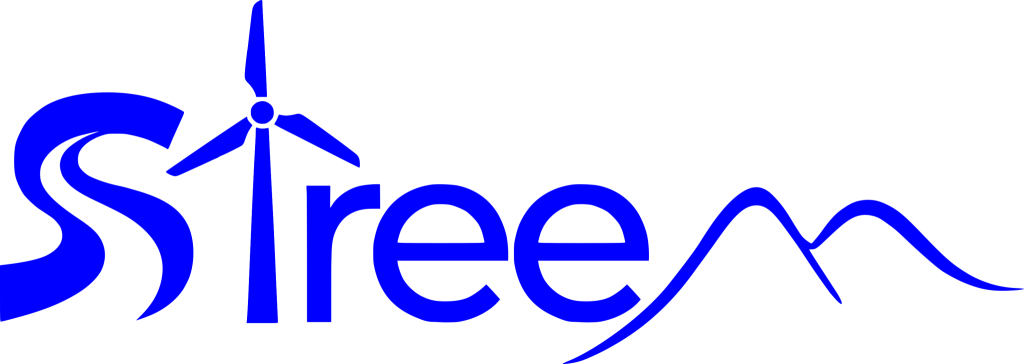
\includegraphics[width=0.4\linewidth]{media/streem.png}
    %\includegraphics[width=0.3\linewidth]{media/EPFLlogo.png}
}
\covercontent{
    \begin{figure}[H]
        \centering
        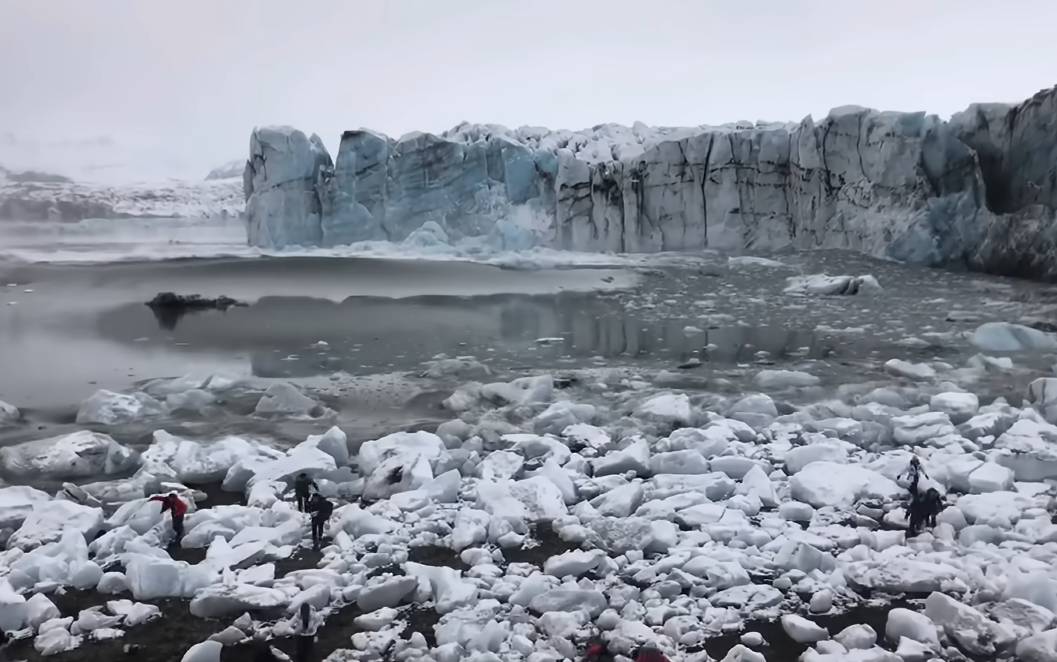
\includegraphics[width=\linewidth]{media/outburst.png}
        \caption{Tourists fleeing an impulse wave caused by a glacier outburst.\\\href{https://www.youtube.com/watch?v=szKtDqmlsH4}{euronews}}
        \label{fig:glof}
    \end{figure}
}

\begin{document}

\makecover

\hypertarget{abstract}{%
\section{Abstract}\label{abstract}}

Impulse waves have been studied at laboratory scale for various speeds,
depths, slopes and materials. As the studied variables are mostly about
the slide, we compare the effects of the topography's shape to the
slide's Froude number.

\begin{quote}
Keywords : Impulse waves, topography, Full factorial design,
multiplicative framework
\end{quote}

\hypertarget{introduction}{%
\section{Introduction}\label{introduction}}

An avalanche generates an \emph{impulse wave} when it strikes a body of
water such as a lake. This wave may damage areas near the lake or
downstream depending on its amplitude. Although it seems like a distant
and excessively rare phenomenon, thousands of people have been killed in
recent history \citep{Vajont, Palcacocha} and even the Léman's tsunami
in the year 563 might have been caused by an impulse wave.

Recent small-scale experiments have studied the effects of the
avalanche's characteristics on the wave's shape. We hereby complement
the recent studies by addressing the effect of topography.

\hypertarget{state-of-the-art}{%
\subsection{State of the art}\label{state-of-the-art}}

Previously, the only method available to estimate the height of an
impulse wave was an empirical relation
(\href{https://www.youtube.com/watch?v=QHvx1SKdqcw}{large and laboratory
scale experiments}), derived from dimensional analysis and focused on
heavy flows such as landslides and debris flows \citep{heller}. This
relation has led to unrealistic predictions in engineering as its
parameter space has not been fully explored yet.

\begin{figure}
\hypertarget{fig:simulation}{%
\centering
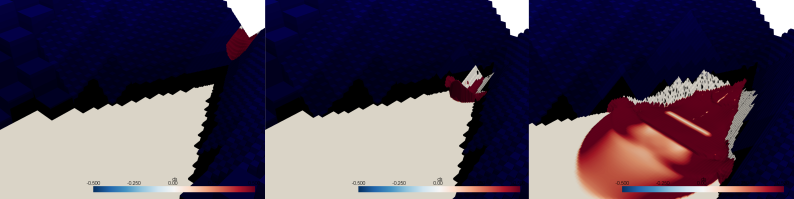
\includegraphics[width=1\textwidth,height=\textheight]{media/s.png}
\caption{Numerical simulation of an impulse wave showing the
free-surface elevation variation at times \(t=1.1~\mathrm{s}\),
\(t=2.2~\mathrm{s}\) and \(t=7.8~\mathrm{s}\).}\label{fig:simulation}
}
\end{figure}

Given this shortcoming, an alternate method was proposed to estimate the
height of impulse waves, in the particular case of snow avalanches
\citep{giboul}. It assumes a sudden transformation of the snow into
water, a supercritical flow (where advection is faster than diffusion)
and relies on a numerical solver to account for a complex topography.
This differs from the scaled experiments in the sense that they could
only test basic topographies. This method was applied to the future
Trift dam \citep{manso, giboul} to forecast the impulse waves and ensure
they will not jump over the dam and destroy the valley. It will serve as
the ground truth for the present study.

\hypertarget{objective}{%
\subsection{Objective}\label{objective}}

In this project, we put aside the avalanche's details to focus on the
effect of topography. To that end, we simulate avalanches with a
numerical model with varying bed slope, bathymetry (submerged
topography) curvature and confinement (how steep the banks are).

\hypertarget{model}{%
\section{Model}\label{model}}

In straight flumes, it has been established that the ratio
\(\eta = h_\mathrm{avalanche}/h_\mathrm{wave}^\mathrm{max}\) scales as

\[
\left(\frac{h_\mathrm{avalanche}}{h_\mathrm{wave}^\mathrm{max}}\right)^{5/4} = \frac{4}{9}\frac{u}{\sqrt{g h}}\cdot\sqrt{\frac{h_s}{h}}\cdot\sqrt[4]{\frac{V_s}{w \ell_s h}}\cdot\sqrt{\cos \phi}
\tag{1}
\]

We wish to extend this result to more complex topographies like narrow
paths or curved bathymetries. To that end, we consider not a straight
slope but one with curvature \(\varsigma\) and a confinement \(\beta\).
They are introduced as dimensionless variables and simply appended to
the product.

\[
\eta = \frac{h_\mathrm{wave}^\mathrm{max}}{h_\mathrm{avalanche}} \propto \mathrm{Fr}^a \cdot \left(\cos\phi\right)^b \cdot \left(\tan{\beta}\right)^c \cdot \varsigma^d \cdot \left(\frac{h_s}{h}\right)^e \cdot \left(\frac{V_s}{V_\ast}\right)^f
\]

However, as avalanches are assumed to follow scale-invariance, a single
avalanche volume is implemented. Moreover, the characteristic depth
\(h\) is meaningless for curved topographies. The same stands for the
relative depth \(h_s/h\). For the same reason, Froude's number has to be
redefined, the avalanche's Froude number is chosen
\(\mathrm{Fr}_s \doteq u / \sqrt{gh_s}\). Finally, we are interested in
finding the coefficients of a widely different system (only the slope
and the slide's speed remain untouched) :

\[
\eta \propto \mathrm{Fr}_s^a \cdot \left(\cos\phi\right)^b \cdot \left(\tan\beta\right)^c \cdot \varsigma^d. \tag{2}
\]

The curvature parameter is arbitrarily set to \(\varsigma\doteq R/h_s\)
where \(R\) is the radius of the circle tangent to the topography.

When working in a log-log framework, this product becomes a linear
relationship :

\[
\ln\eta = \ln\eta_0 + a\ln\mathrm{Fr}_s+b\ln(\cos\phi)+c\ln \left(\tan\beta\right)+d\ln\varsigma.
\]

For the sake of readability, we will write these terms as :

\[
L_X \doteq \frac{\ln(X)-\ln(X_\mathrm{mid})}{\ln(X_\mathrm{max}) - \ln(X_\mathrm{min})} \in [-1, 1]
\]

\[
\Rightarrow L_\eta = L_0 + aL_F + bL_\phi + cL_\beta + dL_\varsigma
\]

\begin{figure}
\hypertarget{fig:bc}{%
\centering
\includesvg[width=1\textwidth,height=\textheight]{media/bc.svg}
\caption{Cross-sections of three avalanches (at the boundary condition)
with different confinements \(\beta\) but equal areas and mean depths.
At the highest confinement, the averaged depth is half the maximum
depth.}\label{fig:bc}
}
\end{figure}

\hypertarget{causal-diagram}{%
\subsection{Causal diagram}\label{causal-diagram}}

\begin{figure}
\hypertarget{fig:cd}{%
\centering
\includesvg[width=0.8\textwidth,height=\textheight]{media/causal_diagram.svg}
\caption{Causal diagram. While the confinement factor implies a depth
correction (see \autoref{fig:bc}), the slope might have an important
influence on the slide's speed.}\label{fig:cd}
}
\end{figure}

\hypertarget{matrices}{%
\subsection{Matrices}\label{matrices}}

The matrix of experiments, \(\underline{\underline{E}}\), of a full
factorial design \(2^4\) is as shown in \autoref{fig:E} :

\begin{figure}
\hypertarget{fig:E}{%
\centering
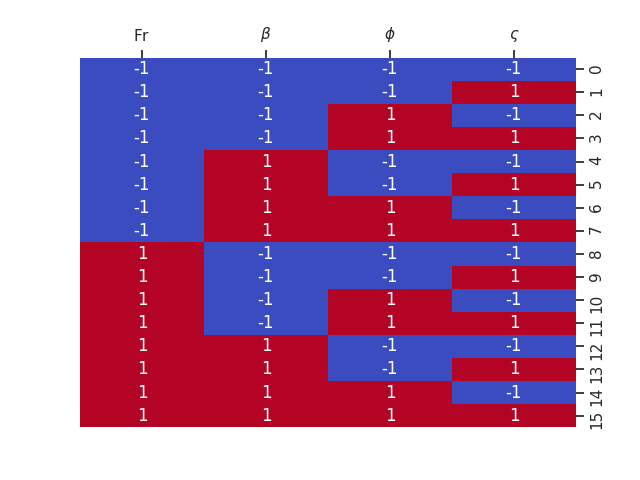
\includegraphics[width=0.5\textwidth,height=\textheight]{media/E.png}
\caption{Matrix of experiment}\label{fig:E}
}
\end{figure}

We chose to do 16 experiments based on how time-consuming the
simulations were. Only two levels are explored (if three were
considered, we woul need 81 experiments ---considerably more).

When incorporating interactions, the model matrix
\(\underline{\underline{M}}\) is as shown in \autoref{fig:M} :

\begin{figure}
\hypertarget{fig:M}{%
\centering
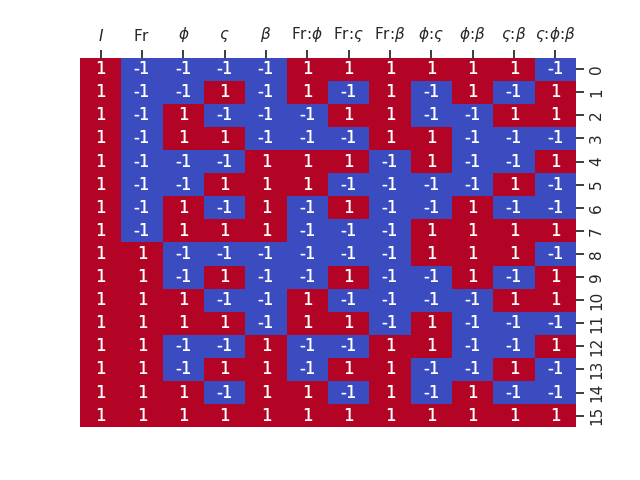
\includegraphics[width=0.6\textwidth,height=\textheight]{media/M.png}
\caption{Model matrix}\label{fig:M}
}
\end{figure}

Thanks to factorial design, the dispersion matrix
\(\underline{\underline{D}}=(\underline{\underline{M}}^T\underline{\underline{M}})^{-1}\)
and variation inflation factor are ideal.

\hypertarget{expected-interactions}{%
\subsection{Expected interactions}\label{expected-interactions}}

As the slide's speed might increase along its run, we expect to see some
interaction between the slope and Froude number.

The modification of the slide's shape by the confinement (see
\autoref{fig:bc}) pushes us to redefine the depth as an average depth. As
this might not be representative of the effective depth, we expect to
see strong interactions with other factors, try though we might by
averaging the depth.

\hypertarget{results}{%
\section{Results}\label{results}}

\hypertarget{linear-model}{%
\subsection{Linear model}\label{linear-model}}

This model is a linearization of equation (2), assuming a linear
combination of all factors.

\[\eta = \eta_0 + a_l\mathrm{Fr} + b_l\cos\phi + c_l\tan\beta + d_l\varsigma\]

By incorporating interactions, we hope to shed light on how orthogonal
our base is.

\[\eta = \eta_0 + \sum_i a_i x_i + \sum_{i,j} a_{ij} x_i x_j\]

Following the execution of our matrix of experiments, the measured
relative effects are shown in \autoref{fig:effects} :

\begin{figure}
\hypertarget{fig:effects}{%
\centering
\includesvg[width=0.8\textwidth,height=\textheight]{media/relative_effects.svg}
\caption{Relative effects.}\label{fig:effects}
}
\end{figure}

It turns out that the confinement factor is null and interactions up to
a third of the slope's factor.

By stacking all contributions with their minimum value as the baseline,
we can see the importance of each factor. The three most important
factors are the Froude number \(\mathrm{Fr}\), the slope \(\phi\) and
the curvature \(\varsigma\).

\begin{figure}
\hypertarget{fig:contrib}{%
\centering
\includesvg[width=1\textwidth,height=\textheight]{media/contributions.svg}
\caption{Contributions from each variable.}\label{fig:contrib}
}
\end{figure}

Once summed up, the interactions do amount to a large part of the result
(see highest and lowest values for \(\eta\) in \autoref{fig:contrib} ).
Overall, the results are satisfying to an environmental hydraulics
engineer. The \autoref{fig:planes} shows planes which are representations
of the predicted field according to our linear model.

\begin{figure}
\hypertarget{fig:planes}{%
\centering
\includesvg[width=0.8\textwidth,height=\textheight]{media/planes.svg}
\caption{Visualizing the main effects.}\label{fig:planes}
}
\end{figure}

\hypertarget{multiplicative-model}{%
\subsection{Multiplicative model}\label{multiplicative-model}}

Falling back to the dimensional analysis, it can be turned into a linear
problem by taking the logarithm of equation (2). Let's take advantage
from the previous model and ignore the confinement \(\tan\beta\).

\[\ln\eta = \ln\eta_0 + A L_\mathrm{Fr} + B L_\phi + C L_\varsigma + d\left( L_\mathrm{Fr} +  L_\phi\right) + e\left(L_\mathrm{Fr} +  L_\varsigma\right) + f\left( L_\phi +  L_\varsigma\right)\]

Where each factor represents a power in equation (2). Interactive
factors in the above logarithmic expression are shared exponents in the
base equation.

\[\frac{\eta}{\eta_0} = \mathrm{Fr}^{A+d+e} \left(\cos\phi\right)^{B+d+f} \varsigma^{C+e+f}\]

Again,

\begin{figure}
\hypertarget{fig:effects_log}{%
\centering
\includesvg[width=0.8\textwidth,height=\textheight]{media/relative_effect_loglog.svg}
\caption{Relative effects within the multiplicative
framework.}\label{fig:effects_log}
}
\end{figure}

\begin{figure}
\hypertarget{fig:planes_log}{%
\centering
\includesvg[width=1\textwidth,height=\textheight]{media/planes_loglog.svg}
\caption{Visualizing the main effects in the multiplicative
framework.}\label{fig:planes_log}
}
\end{figure}

\begin{figure}
\hypertarget{fig:contrib_log}{%
\centering
\includesvg[width=1\textwidth,height=\textheight]{media/contributions_loglog.svg}
\caption{Contributions from each variable within the multiplicative
framework.}\label{fig:contrib_log}
}
\end{figure}

This model has a slightly superior performance. It can be mainly seen
thanks to the reduction in the contribution from the interactions as
shown in \autoref{fig:contrib_log} . The Relative effects show the same
reduction in the importance of interactions.

\hypertarget{relative-error}{%
\subsection{Relative error}\label{relative-error}}

Plotting the relative error and the coeficient of determination shows
that the multiplicative (logarithmic) model has a good performance with
just three factors (using only the main factors). The reader is reminded
that the linear model with interactions has ten factors. Even with four,
it is outperformed by the multiplicative model with just its main
effects.

\begin{figure}
\hypertarget{fig:qq}{%
\centering
\includesvg[width=0.8\textwidth,height=\textheight]{media/qq_plot.svg}
\caption{Empirical-Model quatiles plot}\label{fig:qq}
}
\end{figure}

\hypertarget{discussion}{%
\section{Discussion}\label{discussion}}

What comes as a surprise is the low importance of the confinement
factor. At least an notable interaction with the depth (through the
Froude number) was expected but it seems the averaging of the depth is
good enough to account for confinement.

Although the linear model does well, the multiplicative framework has
the advantage of relying on dimensionnal analysis and is more likely to
hold over a larger parameter space.

The exponent for the Froude number differs from equation (1), this is to
be expected as we redefined the length scale. However, the discrepance
between the expected exponent for the slope and the one found here is
large and remains to be explained.

\hypertarget{conclusion}{%
\section{Conclusion}\label{conclusion}}

This project started with two new topographic factors in mind : the
slide's confinement and the bathymetry's curvature. Although the
numerical results make it seems like the former has no effect, it is an
useful result stating that the average depth is the length scale to use
in impulse waves within this parameter space. As for the latter, it is
shown here that it is twice as important as the slope. This is critical
because this parameter has been studied roughly in laboratories, simply
having angled bathymetry and some depth scale that is hard to determine
in a real case scenario.

As for the coefficient of determination of \SI{99.8}{\percent}, it is
important to note that this ideal numerical simulation does not exhibit
as much noise as a real topography would. With this in mind, we propose
pursuing the quantification of the effect of topography found here :

\[\frac{\eta}{\eta_0} \sim \mathrm{Fr}^{0.294} \left(\cos\phi\right)^{0.09} \varsigma^{0.152}\]

With \(\eta_0=\SI{0.720}{\meter}\).

\bibliography{references}
\label{sec:bibliographie}
\addcontentsline{toc}{section}{\bibname}
\thispagestyle{empty}

\end{document}